\documentclass[11pt]{article}
\usepackage[english]{babel}
\usepackage[utf8]{inputenc}
\usepackage{fancyhdr}
\usepackage{graphicx}

\def\Name{Ran Liao}
\def\Topic{Class Diagram}

\title{\textbf{\Topic}}
\author{\Name}
\markboth{Notes on \Topic\ }{Notes on \Topic\ }
\date{\today}
 
\pagestyle{fancy}
\fancyhf{}
\rhead{\date{\today} }
\lhead{Notes on \Topic\ }
\rfoot{\thepage}

\textheight=9in
%\textwidth=6.5in
\topmargin=-.75in
%\oddsidemargin=0in
%\evensidemargin=0in
 
\begin{document}
\maketitle
\noindent\makebox[\linewidth]{\rule[8pt]{5in}{0.5pt}}

\section*{Visibility Prefixes}

\begin{enumerate}
	\item Prefix + indicates that an attribute or operation is \textbf{public}.
	\item Prefix $-$ denotes that the attribute or operation is \textbf{private}.
	\item Prefix \# denotes that the attribute or operation is \textbf{protected}.
\end{enumerate}

\begin{figure}[h]
	\centering
	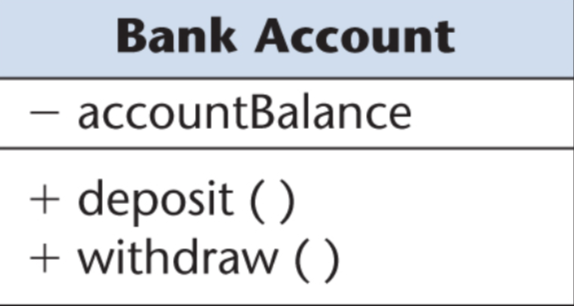
\includegraphics[width=0.3\linewidth]{images/SingleClass.png}
	\caption{Class Diagram Example}
	\label{fig:SingleClass}
\end{figure}

\section*{Aggregation}

Aggregation is the UML term for the part–whole relationship. i.g. A car consists of a chassis, an engine, wheels, and seats. The open diamonds denote aggregation and is placed at the ``whole" end. The numbers next to the ends of the lines denote multiplicity.

\begin{figure}[h]
	\centering
	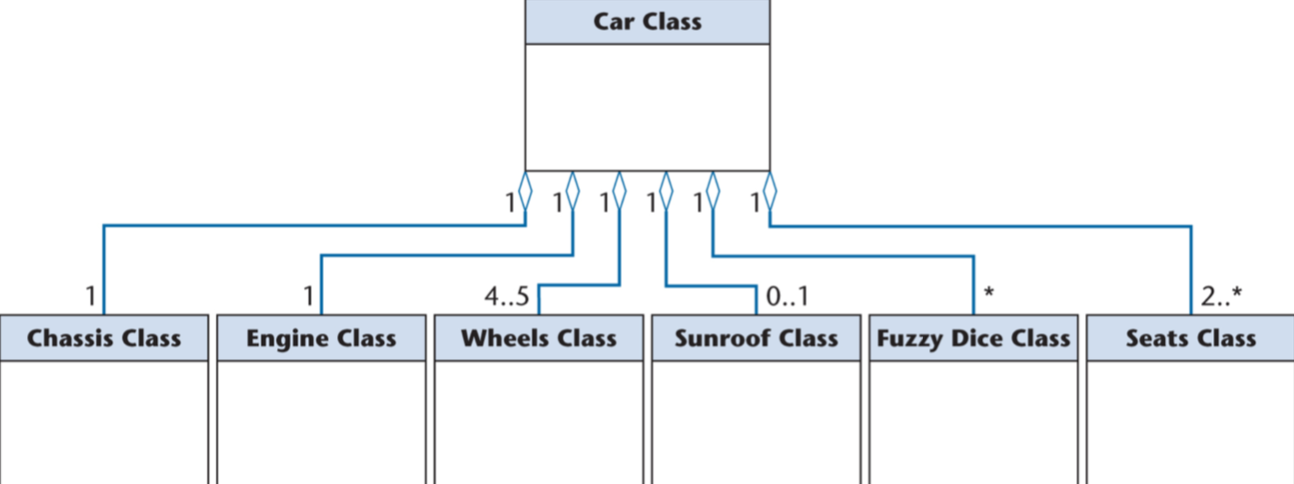
\includegraphics[width=0.9\linewidth]{images/Aggregation.png}
	\caption{Aggregation Relation}
	\label{fig:Aggregation}
\end{figure}


\section*{Composition}

Composition also models the part–whole relationship. However, it is a stronger form of aggregation. Every part may belong to only one whole, and if the whole is deleted, so are the parts. Composition is depicted by a solid diamond.

\begin{figure}[h]
	\centering
	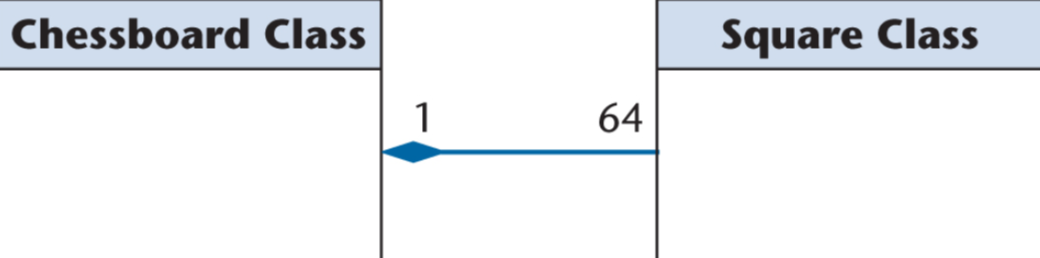
\includegraphics[width=0.5\linewidth]{images/Composition.png}
	\caption{Composition Relation}
	\label{fig:Composition}
\end{figure}

\section*{Generalization}

The UML notation for generalization is an open triangle and sometimes it is labeled with a discriminator.

\begin{figure}[h]
	\centering
	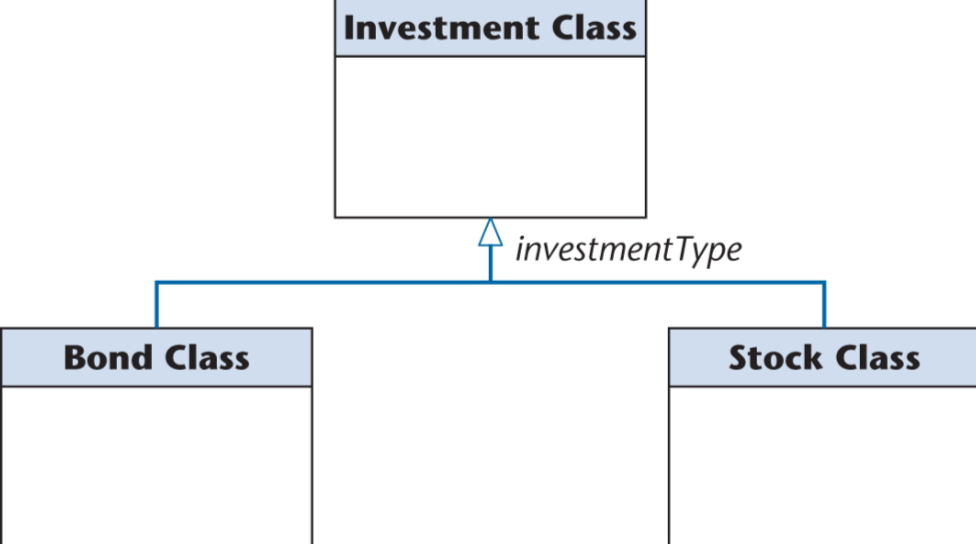
\includegraphics[width=0.5\linewidth]{images/Generalization.png}
	\caption{Generalization Relation}
	\label{fig:Generalization}
\end{figure}

\section*{Association}

The optional navigation triangle shows the direction of the association. And the association between the two classes may be modeled as a class.


\begin{figure}[h]
	\centering
	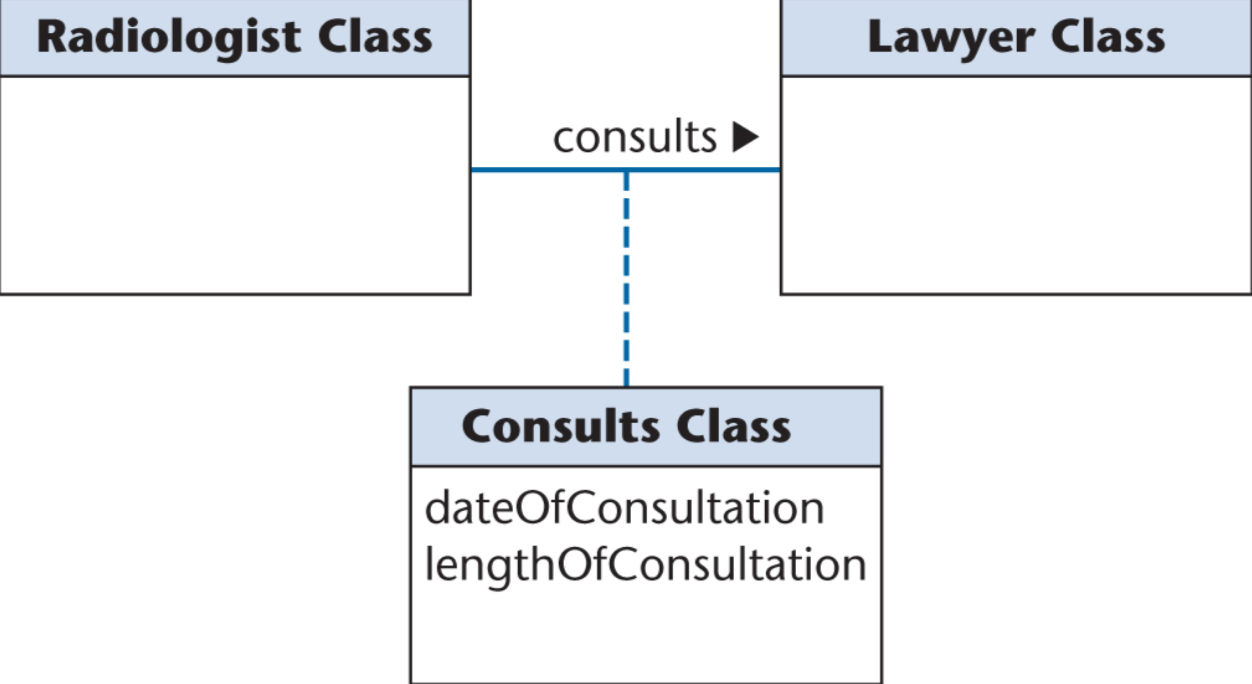
\includegraphics[width=0.5\linewidth]{images/Association.png}
	\caption{Association Relation}
	\label{fig:Association}
\end{figure}







\end{document}